\item \subquestionpointscodingandwritten{4} {\bf Overfitting with expressive models and small data}

For the rest of the problem, we will consider a small
dataset (a random subset of the dataset you have been using so far) with much fewer examples, provided in
the following file:
%
\begin{center}
	\texttt{src/featuremaps/small.csv}
\end{center}
%

We will be exploring what happens when the number of features start becoming bigger than the number of 
examples in the training set. Run your algorithm on this small dataset using the following feature map 
\begin{align}
\phi(x) = \left[\begin{array}{c} 1\\ x \\ x^2\\ \vdots \\x^k \end{array}\right]\in \mathbb{R}^{k+1} 
\end{align}
with $k = 1,2,5,10,20$. 

To verify a correct implementation, consider creating a plot of the various hypothesis curves (just like previous sub-questions, both with and without the sinusoidal features). Observe how the fitting of the training dataset changes as $k$ increases.

\textbf{Remark: } The phenomenon you observe where the models start to fit the training dataset very well, but suddenly ``goes wild'' is due to what is called \emph{overfitting}. The intuition to have for now is that, when the amount of data you have is small relative to the expressive capacity of the family of possible models (that is, the hypothesis class, which, in this case, is the family of all degree $k$ polynomials), it results in overfitting.  

Loosely speaking, the set of hypothesis function is ``very flexible'' and can be easily forced to pass through all your data points especially in unnatural ways. In other words, the  model explains the noises in the training dataset, which shouldn't be explained in the first place. This hurts the predictive power of the model on test examples. We will describe overfitting in more detail in future lectures when we cover learning theory and bias-variance tradeoffs.\\

Your plot should look similar to the following (only polynomial features are shown):
\begin{figure}[H]
  \centering
  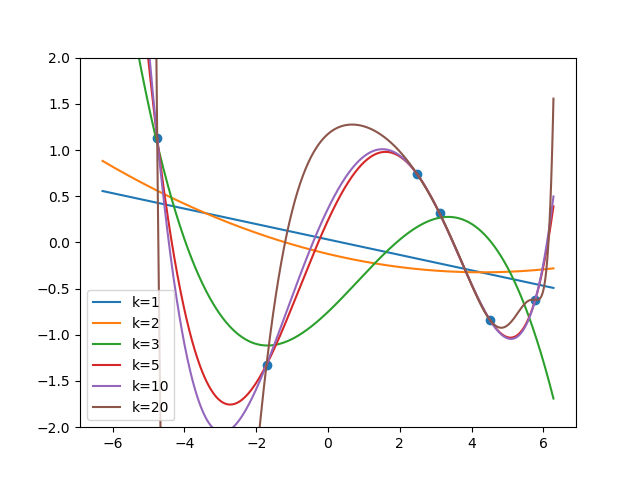
\includegraphics[width=0.65\linewidth]{featuremaps/src/small-poly.png}
  \caption{Polynomial regression with kernel sizes 1,2,3,5,10 and 20
  on small dataset}
\end{figure}

Provide your observations of how the value of k fits the smaller training set here:

\hl{
	With a smaller training set and large k values, we run into the risk of overfitting the data. Given small training data and large k's, the model fits a high order polynomial to the dataset. In other words, what we're seeing is the model giving weights to features that it would have reduced weights to given a larger dataset. Due to the small dataset, the model is not able to recognizes a bad feature and ends up giving it more weight, which yields bad predictions due to overfitting.
}
